\chapter{Evaluation and Results}
\label{chap:evaluation}

\section{Introduction}

This chapter evaluates AURA-MAS as a system. It uses a controlled architectural ablation over nine replay scenarios to address RQ1--RQ5. The chapter sets out the experiment, the metrics, the statistical procedure, the results, and the limits of the evidence.

\begin{revisionbox}
	The first compiled version reported one run of \texttt{demo\_site\_01} and concluded that auction coordination improved precision and halved false alerts. The later 373-run campaign (\texttt{results/evaluation\_campaign\_v2\_notes.md}) does not support that conclusion. Section~\ref{sec:stats_method} shows that no pairwise architecture difference survives correction for multiple comparisons. The coordination and multimodal-fusion claims are corrected in Sections~\ref{sec:c2_retraction} and \ref{sec:rq3}; Appendix~\ref{app:corrections} records each replacement.
\end{revisionbox}

\section{Experimental Setup}

\subsection{Evaluation Methodology}

Component metrics such as \gls{map} and tracking HOTA do not describe the whole alerting system. Operators encounter alert delay, false alerts, and the cost of coordination. Following ETISEO \cite{nghiem2007etiseo} and MLOps evaluation practice \cite{aicity2025, ruf2021demystifying}, the experiment replays recorded sources through the complete agent stack and scores emitted alerts against a ground-truth manifest. Each variant receives the same recorded input. This controls the input, although Section~\ref{sec:threats} explains why it does not fully isolate architecture.

\subsection{Scenario Corpus}
\label{sec:corpus}

Evaluation uses nine scenario manifests rather than the single demonstrator scenario of the first version. Each manifest declares its sensors, zone polygons, and ground-truth incident intervals; full listings appear in Appendix~\ref{app:scenarios}. Table~\ref{tab:corpus} summarizes the corpus.

\begin{table}[H]
	\centering
	\caption{Scenario corpus. Sources are real, citably-licensed recordings (Appendix~\ref{app:datasets}); \texttt{loitering\_01} is a deliberate true-negative probe with empty ground truth.}
	\label{tab:corpus}
	\small
	\begin{tabular}{lccp{5.2cm}}
		\toprule
		\textbf{Scenario}                   & \textbf{Sensors} & \textbf{GT} & \textbf{Purpose / source}                                         \\
		\midrule
		\texttt{intrusion\_01}              & 2 cam, 1 mic     & 2           & Zone intrusion + audio; pedestrian footage                        \\
		\texttt{demo\_site\_01}             & 2 cam, 1 mic     & 3           & Multi-zone demonstrator (\S\ref{sec:demo_case})                   \\
		\texttt{combined\_audio\_video\_01} & 1 cam, 1 mic     & 2           & Cross-modal corroboration probe                                   \\
		\texttt{abandoned\_object\_01}      & 1 cam            & 1           & Static-object rule; ABODA                                         \\
		\texttt{fight\_01}                  & 1 cam            & 1           & CLIP semantic anomaly; AIRTLab \cite{bianculli2020violence}       \\
		\texttt{audio\_glass\_break\_01}    & 1 mic            & 1           & Audio-only, \emph{security} family; ESC-50 \cite{piczak2015esc50} \\
		\texttt{audio\_alarm\_siren\_01}    & 1 mic            & 1           & Audio-only, \emph{hazard} family; ESC-50                          \\
		\texttt{audio\_alarm\_clock\_01}    & 1 mic            & 1           & Audio class discrimination; ESC-50                                \\
		\texttt{loitering\_01}              & 1 cam            & \textbf{0}  & True-negative probe; false-alert floor                            \\
		\bottomrule
	\end{tabular}
\end{table}

The corpus combines three audio-only scenarios, five video-only or video-dominant scenarios, and one cross-modal scenario. Aggregate means therefore mix settings in which different modalities carry the signal. The corpus also has only nine scenarios. Section~\ref{sec:power} shows what that sample size can support.

\subsection{Architecture Variants}

Four variants are compared:

\begin{itemize}
	\item \textbf{Centralized}: a single sequential process iterating over sensors---the classical VMS analytics topology (baseline for RQ1);
	\item \textbf{MAS-nocoord}: concurrent agents, fusion and policy active, coordination disabled (baseline for RQ2);
	\item \textbf{MAS-rules}: coordination via round-robin task assignment (non-market baseline for RQ2);
	\item \textbf{MAS-auction}: the full AURA-MAS design with sealed-bid verification auctions.
\end{itemize}

The first version described the variants as differing only in architecture. That is not accurate. The centralized variant runs sequentially and without pacing, which changes the effective duration of the wall-clock fusion window and alert cooldown. Section~\ref{sec:threats} discusses this pacing confound.

Runs were executed on a 4-vCPU CPU-only sandbox (YOLO11n at 5~\gls{fps} per camera).

\subsection{Campaign Structure}

The campaign crosses scenario, mode, modality configuration, audio backend, and repetition. \texttt{aura\_mas/scripts/run\_campaign.py} starts a fresh subprocess for each run (Figure~\ref{fig:campaign_grid}) because model, tracker, and thread-pool state do not reset reliably in one process. The campaign completed 373 runs without a failure. The main analysis uses the 180 audio-visual YAMNet runs with $N=5$ repetitions.

\begin{figure}[H]
	\centering
	\resizebox{\textwidth}{!}{\input{Assets/tikz/fig_campaign_grid.tex}}
	\caption{Evaluation campaign grid and scoring pipeline. Contribution C5 is this apparatus, not any particular number it produced.}
	\label{fig:campaign_grid}
\end{figure}

\subsection{Metrics}

An alert matches a ground-truth incident if it carries the same incident \emph{family} (Appendix~\ref{app:config}) and falls within a $\pm 5$~s tolerance of the incident interval. We report event-level \textbf{precision, recall, and F1}; \textbf{mean time-to-alert} (TTA); \textbf{false alerts per hour} (FA/h); and \textbf{coordination overhead} (count of task/bid/award/verification messages). Section~\ref{sec:threats} documents three measurement limitations of this scheme---family-level matching, greedy assignment, and the FA/h denominator---each of which bounds what the corresponding number can mean.

\subsection{Statistical Methodology}
\label{sec:stats_method}

The first version of this chapter reported means and standard deviations over $N=5$ repetitions with no interval, test, or effect size. That is insufficient here for a specific reason: on scenarios carrying one to three ground-truth events, per-run F1 takes few distinct values, so a reported ``$0.800\pm0.447$'' describes an outcome that was $1.0$ in four runs and $0.0$ in one---a Bernoulli flip, not a dispersion estimate.

The campaign grid is a \emph{paired} design: every (scenario, repetition) cell is observed under all four modes on identical inputs. The analysis therefore uses the paired difference as its unit and applies:

\begin{itemize}
	\item \textbf{Wilcoxon signed-rank tests} on matched (scenario, repetition) pairs, rather than a paired $t$-test, because per-run F1 is discrete and bounded;
	\item \textbf{Holm--Bonferroni correction} across all six pairwise mode comparisons---quoting the smallest of six uncorrected $p$-values would be a multiplicity error;
	\item \textbf{Cliff's $\delta$} as a non-parametric effect size, reported alongside every $p$-value;
	\item \textbf{Bootstrap percentile confidence intervals} (10{,}000 resamples, fixed seed) on per-mode means and on paired differences.
\end{itemize}

All values are produced by \texttt{aura\_mas/scripts/thesis\_stats.py} into \texttt{results/thesis\_stats.json} and emitted directly as \LaTeX{} tables, so no number in this chapter is transcribed by hand. The analysis set comprises $n=45$ fully-observed paired cells (9 scenarios $\times$ 5 repetitions).

\section{Results}
\label{sec:ablation}

\subsection{Architectural Ablation Across the Corpus}

Table~\ref{tab:per_scenario_f1} reports event-level F1 for every scenario and mode; Figure~\ref{fig:per_scenario_f1} presents the same data as a heatmap.

\begin{table}[H]
	\centering
	\caption{Event-level F1 per scenario and architecture (mean$\pm$sd over $N=5$ repetitions, YAMNet backend). Bold marks the best mode per scenario. $^{\dagger}$\texttt{loitering\_01} has empty ground truth by construction, so F1 is 0 for every mode.}
	\label{tab:per_scenario_f1}
	\scriptsize
	% GENERATED by aura_mas/scripts/thesis_stats.py -- do not edit by hand.
\begin{tabular}{lcccc}
\toprule
\textbf{Scenario} & \textbf{Centralized} & \textbf{MAS-nocoord} & \textbf{MAS-rules} & \textbf{MAS-auction} \\
\midrule
\texttt{abandoned\_object\_01} & \textbf{0.667$\pm$0.000} & 0.534$\pm$0.298 & 0.200$\pm$0.447 & 0.200$\pm$0.447 \\
\texttt{audio\_alarm\_clock\_01} & \textbf{1.000$\pm$0.000} & \textbf{1.000$\pm$0.000} & \textbf{1.000$\pm$0.000} & \textbf{1.000$\pm$0.000} \\
\texttt{audio\_alarm\_siren\_01} & 0.200$\pm$0.447 & 0.600$\pm$0.548 & \textbf{0.800$\pm$0.447} & \textbf{0.800$\pm$0.447} \\
\texttt{audio\_glass\_break\_01} & 0.000$\pm$0.000 & \textbf{0.800$\pm$0.447} & \textbf{0.800$\pm$0.447} & \textbf{0.800$\pm$0.447} \\
\texttt{combined\_audio\_video\_01} & \textbf{0.467$\pm$0.274} & 0.400$\pm$0.224 & 0.200$\pm$0.274 & 0.100$\pm$0.224 \\
\texttt{demo\_site\_01} & 0.773$\pm$0.059 & \textbf{0.781$\pm$0.204} & 0.629$\pm$0.053 & 0.667$\pm$0.000 \\
\texttt{fight\_01} & \textbf{1.000$\pm$0.000} & 0.800$\pm$0.447 & 0.400$\pm$0.548 & 0.200$\pm$0.447 \\
\texttt{intrusion\_01} & \textbf{0.567$\pm$0.091} & 0.280$\pm$0.259 & 0.380$\pm$0.217 & 0.300$\pm$0.274 \\
\texttt{loitering\_01$^{\dagger}$} & 0.000$\pm$0.000 & 0.000$\pm$0.000 & 0.000$\pm$0.000 & 0.000$\pm$0.000 \\
\bottomrule
\end{tabular}

\end{table}

\begin{figure}[H]
	\centering
	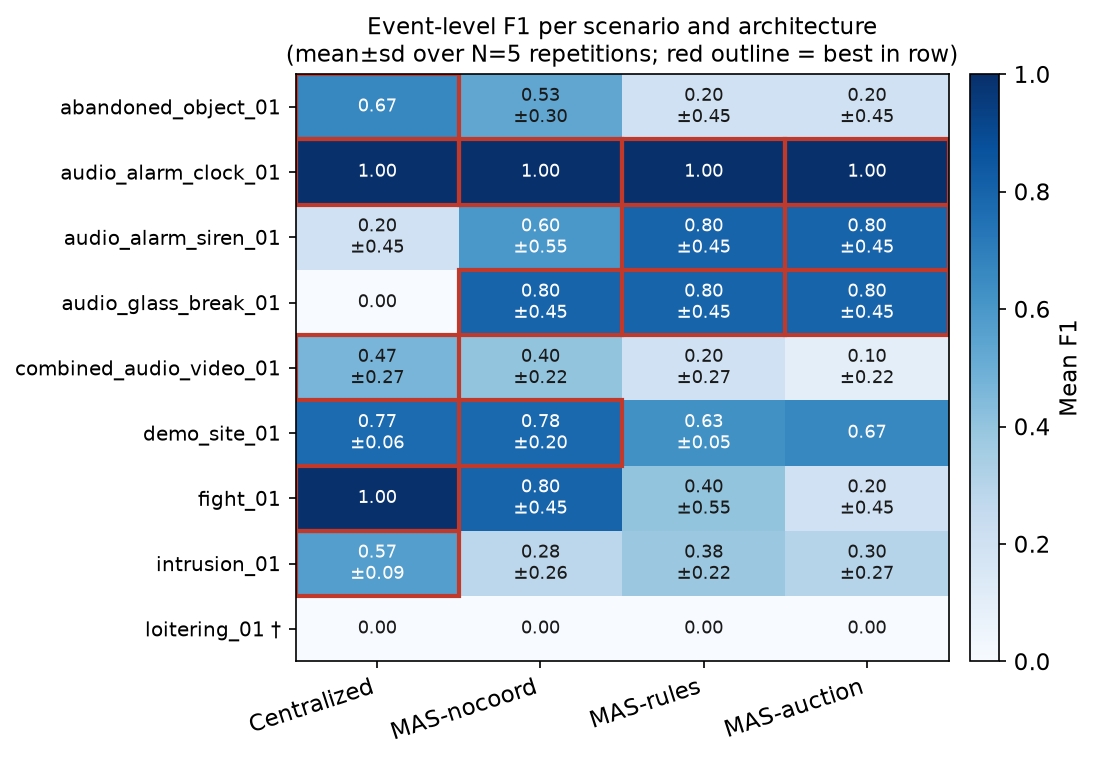
\includegraphics[width=0.88\textwidth]{Assets/fig_per_scenario_f1.png}
	\caption{Event-level F1 across the nine-scenario corpus. No mode dominates: the centralized baseline wins on the video-dominant scenarios, while all three MAS variants win on the audio-only scenarios.}
	\label{fig:per_scenario_f1}
\end{figure}

The per-scenario results depend on the modality carrying the signal. The centralized baseline is best on \texttt{fight\_01}, \texttt{abandoned\_object\_01}, \texttt{intrusion\_01}, and \texttt{combined\_audio\_video\_01}, which are video-dominant scenarios. All three MAS variants beat it on \texttt{audio\_glass\_break\_01} (0.800 vs.\ 0.000) and \texttt{audio\_alarm\_siren\_01}. The overall mean is therefore strongly affected by the corpus's modality mix.

With that caveat stated, the marginal means are given in Table~\ref{tab:marginal_f1} and Figure~\ref{fig:mode_ci}.

\begin{table}[H]
	\centering
	\caption{Marginal mean F1 per mode with bootstrap confidence intervals ($n=45$ paired observations per mode).}
	\label{tab:marginal_f1}
	\small
	% GENERATED by aura_mas/scripts/thesis_stats.py -- do not edit by hand.
\begin{tabular}{lrrrr@{\,}c@{\,}l}
\toprule
\textbf{Mode} & \textbf{$n$} & \textbf{Mean} & \textbf{Median} & \multicolumn{3}{c}{\textbf{95\% CI (bootstrap)}} \\
\midrule
Centralized & 45 & 0.519 & 0.667 & [0.401 & , & 0.633] \\
MAS-nocoord & 45 & 0.577 & 0.667 & [0.455 & , & 0.697] \\
MAS-rules & 45 & 0.490 & 0.500 & [0.361 & , & 0.620] \\
MAS-auction & 45 & 0.452 & 0.500 & [0.322 & , & 0.589] \\
\bottomrule
\end{tabular}

\end{table}

\begin{figure}[H]
	\centering
	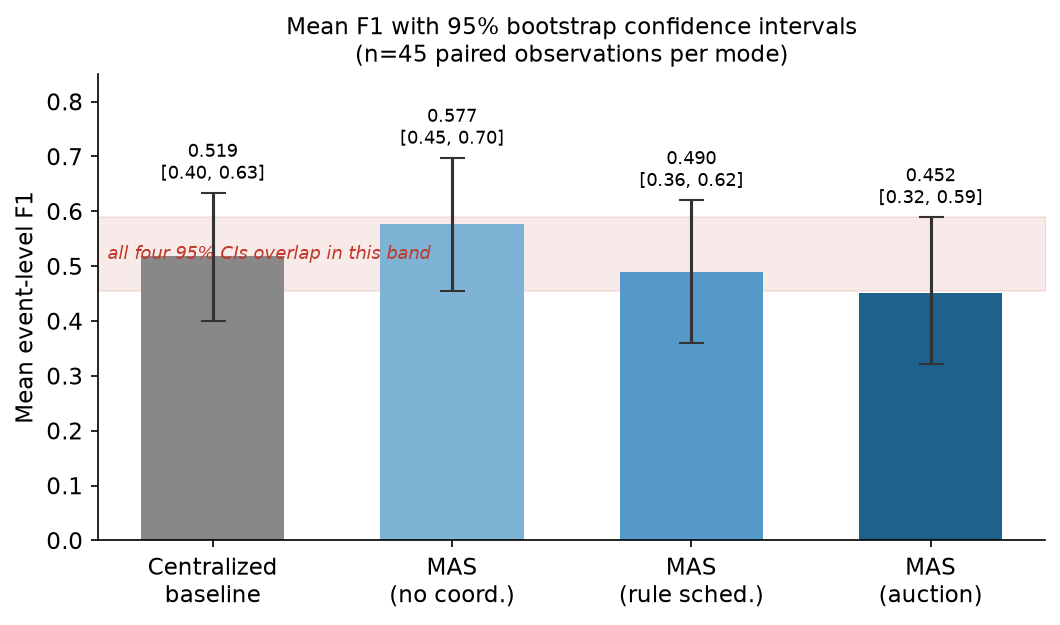
\includegraphics[width=0.78\textwidth]{Assets/fig_mode_ci.png}
	\caption{Mean event-level F1 with 95\% bootstrap confidence intervals. All four intervals overlap in the shaded band.}
	\label{fig:mode_ci}
\end{figure}

On point estimates, the ordering is MAS-nocoord (0.577) $>$ Centralized (0.519) $>$ MAS-rules (0.490) $>$ MAS-auction (0.452). \textbf{The full AURA-MAS configuration has the lowest mean F1 of the four variants on this corpus.} This directly contradicts the first version's conclusion and is reported here as the primary result.

\subsection{Inferential Analysis}
\label{sec:power}

Point-estimate orderings over 45 observations invite over-reading, so Table~\ref{tab:pairwise_f1} gives the paired tests and Figure~\ref{fig:paired_forest} the corresponding intervals.

\begin{table}[H]
	\centering
	\caption{Pairwise architecture comparisons on F1, paired on (scenario, repetition). $\Delta$~mean is mode~A minus mode~B; $\delta$ is Cliff's delta; $p_{\text{Holm}}$ is Holm--Bonferroni-adjusted across all six comparisons.}
	\label{tab:pairwise_f1}
	\scriptsize
	% GENERATED by aura_mas/scripts/thesis_stats.py -- do not edit by hand.
\begin{tabular}{llrr@{\,}c@{\,}lrrr}
\toprule
\textbf{Mode A} & \textbf{Mode B} & \textbf{$\Delta$ mean} & \multicolumn{3}{c}{\textbf{95\% CI}} & \textbf{$p$} & \textbf{$p_{\text{Holm}}$} & \textbf{$\delta$} \\
\midrule
MAS-nocoord & MAS-auction & +0.125 & [0.022 & , & 0.229] & 0.024 & 0.145 & +0.146 \\
MAS-nocoord & MAS-rules & +0.087 & [-0.015 & , & 0.189] & 0.097 & 0.487 & +0.107 \\
Centralized & MAS-nocoord & -0.058 & [-0.205 & , & 0.082] & 0.432 & 1.000 & -0.085 \\
MAS-rules & MAS-auction & +0.038 & [-0.066 & , & 0.144] & 0.552 & 1.000 & +0.044 \\
Centralized & MAS-auction & +0.067 & [-0.113 & , & 0.239] & 0.562 & 1.000 & +0.067 \\
Centralized & MAS-rules & +0.029 & [-0.136 & , & 0.189] & 0.671 & 1.000 & +0.028 \\
\bottomrule
\end{tabular}

\end{table}

\begin{figure}[H]
	\centering
	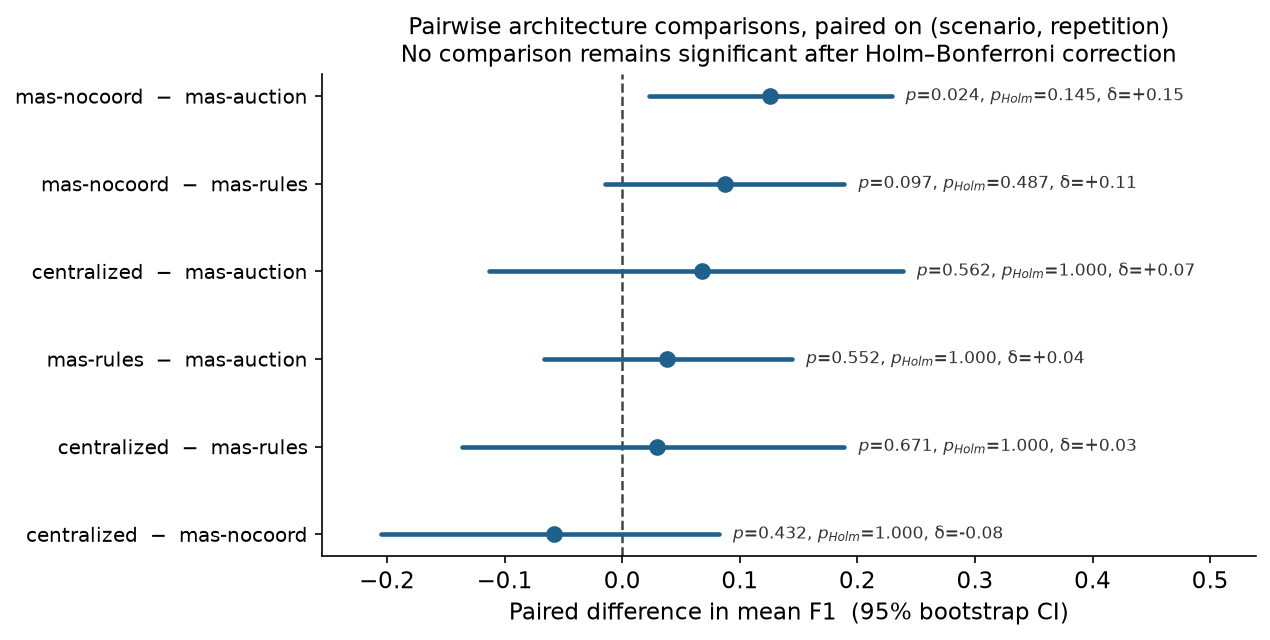
\includegraphics[width=0.95\textwidth]{Assets/fig_paired_forest.png}
	\caption{Paired mean differences in F1 with 95\% bootstrap confidence intervals. Every interval either contains zero or, after multiplicity correction, cannot be distinguished from it.}
	\label{fig:paired_forest}
\end{figure}

\begin{findingbox}[title={Principal empirical finding}]
	Across the nine-scenario corpus, \textbf{none of the six pairwise architecture comparisons on F1 is statistically significant after Holm--Bonferroni correction}. The largest raw effect---MAS-nocoord over MAS-auction, $\Delta=+0.125$, $p=0.024$---becomes $p_{\text{Holm}}=0.145$, with Cliff's $\delta=+0.146$, a negligible effect size. All four bootstrap confidence intervals overlap substantially.

	This campaign cannot distinguish the four architectures on detection quality. The point-estimate ordering should not be read as a performance ranking.
\end{findingbox}

For the observed MAS-nocoord/MAS-auction difference, the standardized paired effect size is $d_z=0.35$. Detecting an effect of that size with 80\% power at $\alpha=0.05$ requires about \textbf{65 paired observations}; this campaign has 45 (Figure~\ref{fig:power_curve}). At five repetitions per scenario, that corresponds to about \textbf{13 scenarios}, not nine. A larger corpus is needed before treating the ordering as evidence of an architecture effect.

\begin{figure}[H]
	\centering
	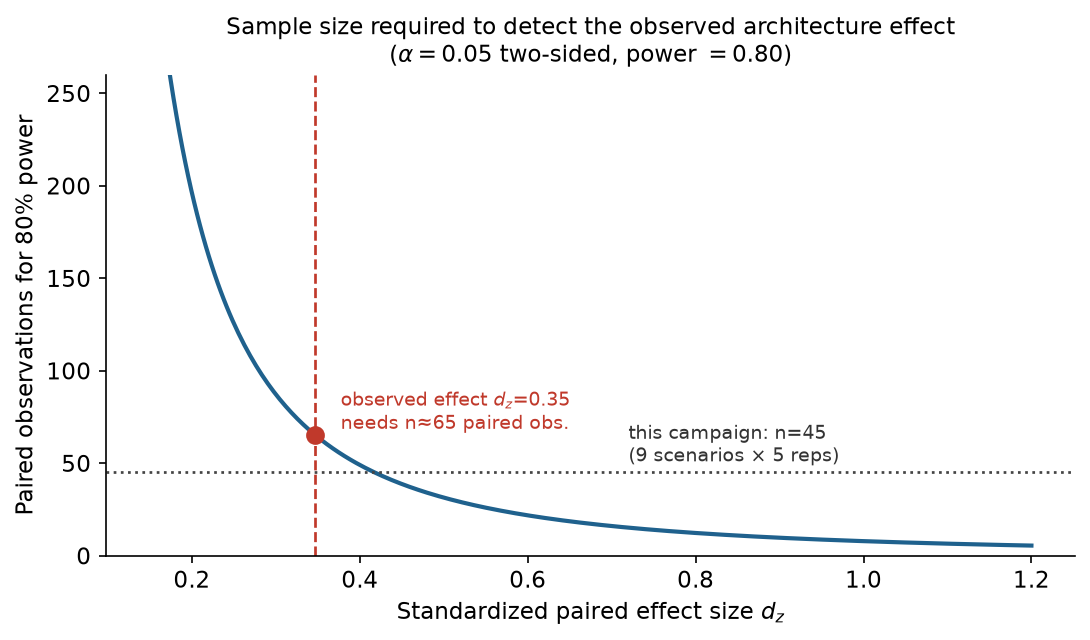
\includegraphics[width=0.76\textwidth]{Assets/fig_power_curve.png}
	\caption{Paired observations required for 80\% power as a function of standardized effect size, with this campaign's position marked.}
	\label{fig:power_curve}
\end{figure}

A sensitivity check excluding the empty-ground-truth \texttt{loitering\_01} probe leaves the conclusion unchanged: the means rise (nocoord 0.649, centralized 0.584, rules 0.551, auction 0.508) but no comparison becomes significant after correction (\texttt{results/thesis\_stats.json}, key \texttt{sensitivity\_excluding\_probe}).

\subsection{Audio Backend Ablation: DSP Fallback vs.\ YAMNet}
\label{sec:audio_ablation}

The one manipulation in this campaign with an unambiguous effect is the audio backend. Replaying the three audio-only scenarios under both backends ($N=3$ per cell), the \gls{dsp} fallback scores F1 $=0.000\pm0.000$ in \emph{every} repetition, across all four coordination modes and all three scenarios, while YAMNet reaches $0.6$--$1.0$ on most scenario/mode pairs and a clean $1.000\pm0.000$ on \texttt{audio\_alarm\_clock\_01} (Figure~\ref{fig:audio_backend_ablation}).

\begin{figure}[H]
	\centering
	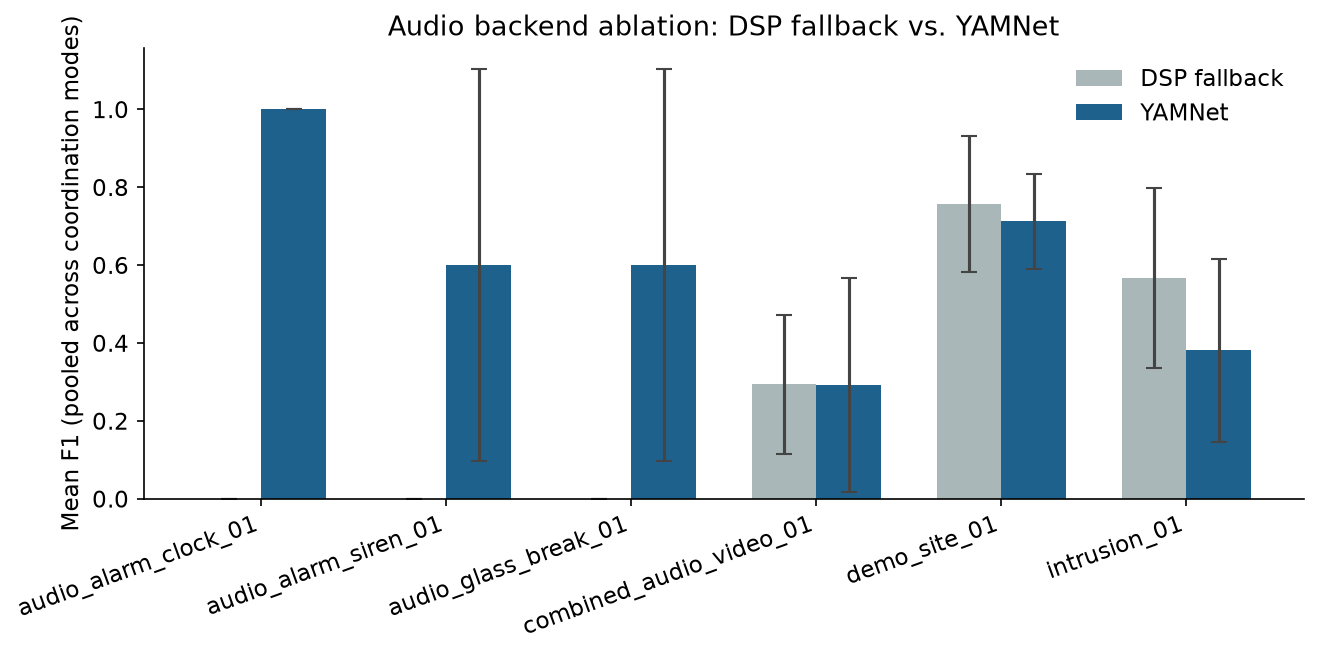
\includegraphics[width=0.85\textwidth]{Assets/fig_audio_backend_ablation.png}
	\caption{F1 by audio backend across the three audio-only scenarios.}
	\label{fig:audio_backend_ablation}
\end{figure}

This is a matching result rather than a direct comparison of audio detection quality. The \gls{dsp} path emits the generic \texttt{audio\_anomaly} type, mapped to the \emph{violence\_or\_hazard} family. The audio-only manifests use \emph{security} and \emph{hazard} ground-truth families. Family-level matching therefore cannot count a \gls{dsp} detection as a true positive, even if it detects the transient. The $0.000$ result shows a label-space mismatch. Under this protocol, class-specific audio typing is required for the modality to score as usable.

\subsection{Analysis by Research Question}

\textbf{RQ1 (Architecture).} On \texttt{demo\_site\_01}, mean TTA falls from $15.07\pm3.11$~s (centralized) to $2.96\pm0.14$~s (MAS-auction), an 80.4\% reduction. That result does not extend to the wider corpus. Across the seven scenarios in which all four modes produce a matched alert, the paired means are centralized 9.47~s, MAS-nocoord 8.87~s, MAS-rules 6.60~s, and MAS-auction 8.46~s. The centralized-to-auction difference is 10.7\%, with $p=0.59$, and no pairwise TTA comparison is significant after correction. \texttt{demo\_site\_01} is the only scenario in which the centralized variant is much slower. Its own $N=5$ result has $p=0.0625$.

\begin{figure}[H]
	\centering
	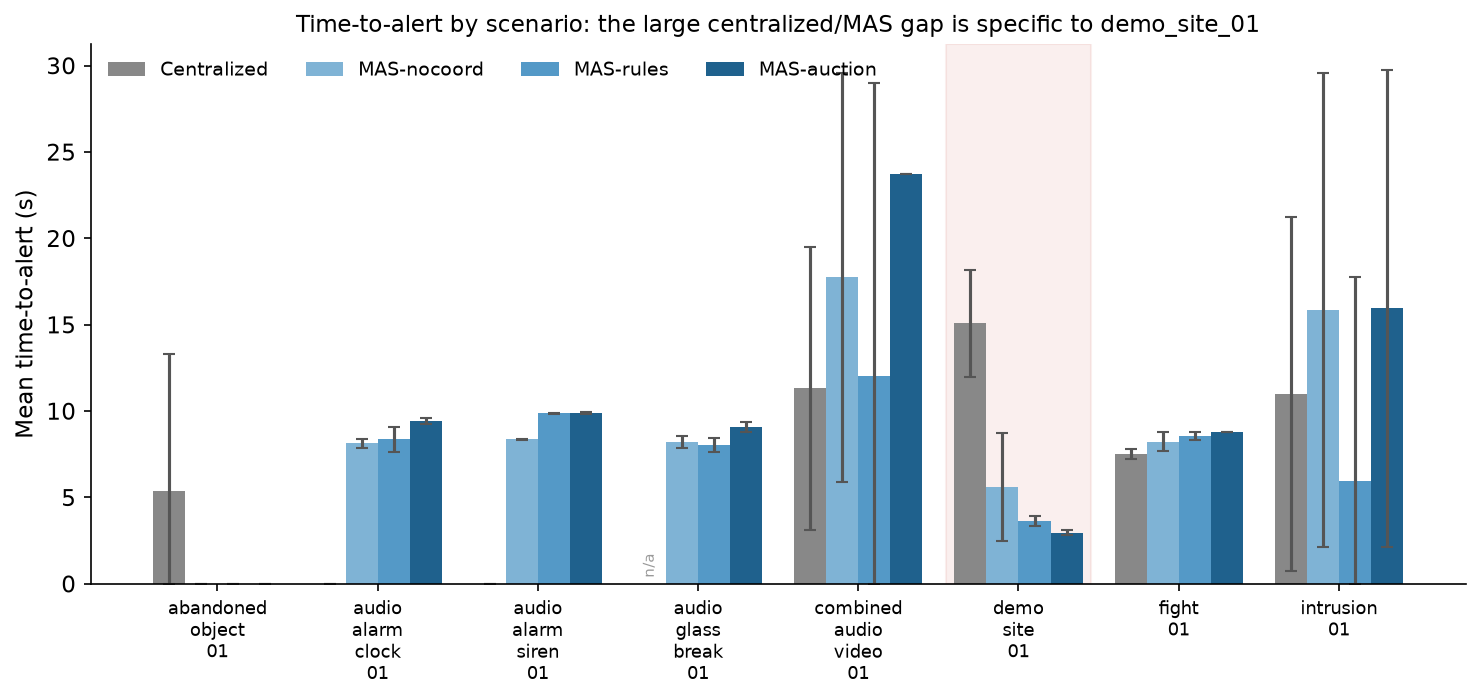
\includegraphics[width=0.97\textwidth]{Assets/fig_tta_per_scenario.png}
	\caption{Mean time-to-alert by scenario. The large centralized/MAS gap is specific to \texttt{demo\_site\_01} (shaded); elsewhere the ordering flattens or reverses. ``n/a'' marks mode/scenario pairs that produced no matched alert.}
	\label{fig:tta_per_scenario}
\end{figure}

Sequential processing can create head-of-line blocking, so a concurrency effect is plausible. Here, however, the result is confounded with pacing and appears clearly in only the scenario with the most sensors. RQ1 remains unresolved.

\textbf{RQ2 (Coordination).} Addressed in Section~\ref{sec:c2_retraction}.

\textbf{RQ3 (Multimodality).}
\label{sec:rq3}
Audio zone tagging and event-family taxonomy unification allow audio and video events to enter the same hypothesis (Chapter~\ref{chap:implementation}). Four campaign alerts list both a camera and a microphone in their \texttt{sensors} field. The mechanism therefore runs end to end.

\begin{revisionbox}
	The first version of this chapter stated that on \texttt{combined\_audio\_video\_01} ``the resulting alert's confidence (0.78) reflects the audio+video corroboration bonus of Equation~\ref{eq:noisyor}.'' \textbf{This is incorrect.} Direct inspection of every alert in the campaign (\texttt{results/cross\_modal\_fusion\_audit.md}) shows that the 0.78 alert carries \texttt{sensors: ["cam\_01"]} and exactly one fused event, so neither bonus term---both gated on $|M(H)|>1$ and $|S(H)|>1$---can apply. The value 0.78 is precisely one unaided video event: $1-(1-0.9\times0.867)=0.780$. All 37 alerts at confidence 0.78 in the campaign are single-sensor.
\end{revisionbox}

Only 4 of 240 alerts are genuinely cross-modal because audio and video events must share a (family, zone) key within the same 6~s window. Their effect on reported confidence cannot be measured because noisy-OR reaches the clamp first. In the example in Figure~\ref{fig:fusion_timeline}, four same-camera detections already produce 0.9992. The two $+0.05$ bonuses are then absorbed by the $[0,1]$ clamp, and a video-only hypothesis reaches the same reported 1.0. All four cross-modal alerts report 1.0.

\begin{figure}[H]
	\centering
	\resizebox{\textwidth}{!}{\input{Assets/tikz/fig_fusion_timeline.tex}}
	\caption{Hypothesis formation and noisy-OR saturation on \texttt{combined\_audio\_video\_01}. Confidences are the values recorded in the run artifacts.}
	\label{fig:fusion_timeline}
\end{figure}

Noisy-OR treats repeated observations of one incident from one sensor as conditionally independent, although they are not. C3's monotonicity guarantee still holds, but the score has already saturated at these event confidences. A later version should pool evidence per sensor or use a dependence-aware combination rule.

Separately, \texttt{Hypothesis.dominant\_type()} labels all four cross-modal alerts \texttt{intrusion} rather than \texttt{audio\_glass\_break}, because video confidence always outscores audio confidence within the merged hypothesis. A reader of the raw alert log therefore sees no indication that audio contributed---a limitation of single-winner event-type labelling that motivates the \texttt{contributing\_types} field discussed in Chapter~\ref{chap:conclusion}.

\textbf{RQ4 (Agentic explanation).}
\label{sec:rq4}
Explanation generation occurs strictly after alert emission by construction, so it cannot affect alerting latency; measured policy decision latency averages 0.3~ms.

\begin{revisionbox}
	The first version stated that ``in replay runs, all accepted reports cited only identifiers present in the event log, i.e., zero uncaught hallucinated citations.'' This claim is \textbf{vacuous as stated}: \texttt{run\_campaign.py} never passes \texttt{--llm}, so across all 373 runs the \gls{llm} path never executed and every \texttt{explanation} field written to disk is the deterministic fallback template (\texttt{results/explanation\_judge\_notes.md}). No report was generated by a model, so none could have been found grounded.
\end{revisionbox}

C4 has structural evidence and one observed model run. The explanation pipeline is a finite state machine (Figure~\ref{fig:explanation_fsm}); every path to \texttt{emitted} passes the guardrail, and every failure uses the deterministic template. Inspection and unit tests can verify that control flow without making claims about a model. In one post-campaign run, a local \texttt{qwen2.5-vl:3b} report failed the guardrail and triggered the template (\texttt{aura.guardrail.passed: false}, \texttt{aura.explanation.fallback\_triggered: true} in \texttt{data/otel\_spans.jsonl}). This single result shows that the mechanism can fire, but it does not evaluate the guardrail or the local model. C4 remains a structural design contribution.

\begin{figure}[H]
	\centering
	\resizebox{0.98\textwidth}{!}{% ============================================================================
% ExplanationAgent finite state machine
% Source of truth: aura_mas/agents/explanation_fsm.py (python-statemachine)
%   states      : collecting (initial), describing, drafting,
%                 checking_guardrail, emitted (final), fallback (final)
%   transitions : collect_done (conditional on use_vision), describe_done,
%                 draft_done, guardrail_passed, guardrail_failed, fail (from
%                 every non-final state)
% Referenced as fig:explanation_fsm.
% ============================================================================
\begin{tikzpicture}[
	font=\small,
	node distance=15mm and 21mm,
	st/.style={draw=black!70, fill=black!4, rounded corners=3pt,
			minimum height=9mm, minimum width=25mm, align=center,
			font=\small},
	final/.style={st, draw=darkgreen!75, fill=darkgreen!8, very thick},
	bad/.style={st, draw=red!70, fill=red!7, very thick},
	tr/.style={-{Latex[length=2.2mm]}, thick, black!75},
	failtr/.style={-{Latex[length=2mm]}, thick, red!65, dashed},
	lbl/.style={font=\scriptsize, inner sep=1.5pt, fill=white},
	ann/.style={font=\scriptsize\itshape, black!55, align=left},
	]

	\node[st] (collect) {\texttt{collecting}\\[-1pt]{\scriptsize\itshape initial}};
	\node[st, right=of collect] (describe) {\texttt{describing}\\[-1pt]{\scriptsize VLM frame caption}};
	\node[st, right=of describe] (draft) {\texttt{drafting}\\[-1pt]{\scriptsize LLM structured report}};
	\node[st, below=18mm of draft] (guard) {\texttt{checking\_guardrail}};
	\node[final, left=34mm of guard] (emit) {\texttt{emitted}\\[-1pt]{\scriptsize\itshape final}};
	\node[bad, below=14mm of guard] (fall) {\texttt{fallback}\\[-1pt]{\scriptsize deterministic template}};

	% happy path
	\draw[tr] (collect) -- node[lbl,above]{\texttt{collect\_done}}
	node[lbl,below]{\scriptsize\texttt{use\_vision}} (describe);
	\draw[tr] (describe) -- node[lbl,above]{\texttt{describe\_done}} (draft);
	\draw[tr] (draft) -- node[lbl,right]{\texttt{draft\_done}} (guard);
	\draw[tr] (guard) -- node[lbl,above]{\texttt{guardrail\_passed}} (emit);
	\draw[tr] (guard) -- node[lbl,left]{\texttt{guardrail\_failed}} (fall);

	% conditional bypass when vision disabled
	\draw[tr] (collect.north) to[out=35,in=145]
	node[lbl,above,pos=0.5]{\texttt{collect\_done} \ \scriptsize\texttt{unless use\_vision}}
	(draft.north);

	% fail edges from every non-final state
	\draw[failtr] (collect.south) to[out=-70,in=170] (fall.west);
	\draw[failtr] (describe.south) to[out=-90,in=150] (fall.north west);
	\draw[failtr] (draft.east) to[out=-40,in=20] (fall.east);

	\node[ann, anchor=north west, text width=13.4cm] at ($(fall.south west)+(-2.9,-0.5)$)
	{Dashed red: the \texttt{fail} transition, available from \emph{every}
		non-final state. No path reaches \texttt{emitted} except through a
		passing guardrail check --- the structural property behind
		contribution~C4. The guardrail rejects any report citing an
		\texttt{evidence\_id} absent from the alert; a structurally invalid
		response is \emph{not} retried, it routes straight to fallback.};

\end{tikzpicture}
}
	\caption{ExplanationAgent state machine (\texttt{aura\_mas/agents/explanation\_fsm.py}). The guardrail is the sole gate on the \texttt{emitted} state.}
	\label{fig:explanation_fsm}
\end{figure}

\textbf{RQ5 (Governance).} This question concerns invariants rather than effect sizes. Every exported crop passed through the anonymization choke point in \texttt{aura\_mas/core/privacy.py}. The campaign wrote 1{,}737 anonymized evidence files, with examples in Figure~\ref{fig:evidence_grid}, and persisted or transmitted no raw frame. Each alert and suppression produced an audit record across all 373 runs, with a separate audit JSONL file for each run.

\begin{figure}[H]
	\centering
	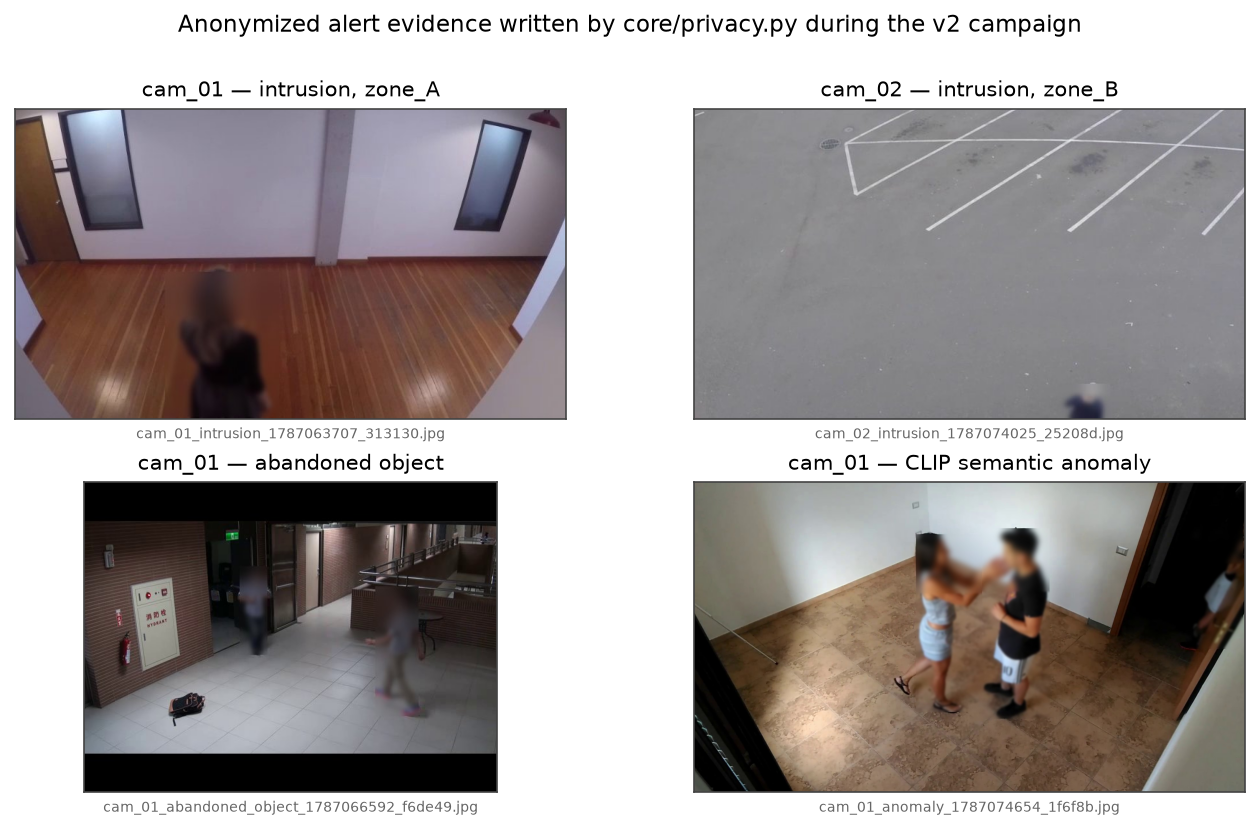
\includegraphics[width=0.94\textwidth]{Assets/fig_evidence_grid.png}
	\caption{Anonymized alert evidence written by the privacy choke point during the campaign. Person regions receive graded Gaussian blurring, strongest over the head region; if no person localization is available the module fails closed and blurs the whole frame. Filenames are retained so any panel can be traced to its run.}
	\label{fig:evidence_grid}
\end{figure}

Two boundaries on this claim should be stated plainly. First, anonymization \emph{efficacy} is asserted structurally---every export traverses the choke point---but never measured; no re-identification attack was attempted against the blurred crops. Second, the audit stream is append-only by convention, not cryptographically immutable; the word ``immutable'' in the first version overstates it, and Chapter~\ref{chap:conclusion} lists hash-chaining as the concrete remedy.

\section{Coordination: Retraction and Reassessment}
\label{sec:c2_retraction}

RQ2 asks whether auction-based verification allocation improves alert precision over uncoordinated alerting, and at what communication cost. This section answers it, and in doing so retracts the first version's central claim for contribution C2.

\subsection{What the first version claimed}

The first version reported, from a single run, that auction coordination halved false alerts and restored precision, and concluded that because MAS-rules and MAS-auction pay a similar message cost, ``the difference is attributable to \emph{who} is asked to verify, not merely that verification happens---validating the utility-bid design in which field-of-view overlap and origin-independence, not an arbitrary rotation, dominate the bid.''

\subsection{Why that claim cannot be supported}

\begin{revisionbox}
	The utility-bid claim is \textbf{retracted}. The bid function is $u = b\cdot\kappa\cdot o$, where $o$ is intended to be the camera's field-of-view overlap with the event zone. In the evaluated code, $o$ is read as \texttt{task.get("fov\_overlap", \{\}).get(self.agent\_id, 0.5)} (\texttt{aura\_mas/agents/camera\_agent.py:448}), and the coordinator never populated \texttt{fov\_overlap} when constructing the task. \textbf{Throughout all 373 runs, $o$ was the constant 0.5 for every camera.}

	The bid therefore reduced to $b\cdot\kappa$: 0.3 for the originating sensor and 1.0 for any other idle camera. On a two-camera site, it deterministically selects the other camera, as round-robin does. The measured code never activates the mechanism needed to test the original claim.
\end{revisionbox}

Figure~\ref{fig:auction_sequence} traces the protocol and marks where the inert term enters. This also explains mechanistically why MAS-auction and MAS-rules produce statistically indistinguishable results ($\Delta=+0.038$, $p_{\text{Holm}}=1.000$, $\delta=+0.044$): under an inert overlap term on a two-camera site, they are close to the same allocator.

\begin{figure}[H]
	\centering
	\resizebox{\textwidth}{!}{\input{Assets/tikz/fig_auction_sequence.tex}}
	\caption{Auction-based active verification message sequence, annotated with the measurement caveat that the overlap term was inert during evaluation.}
	\label{fig:auction_sequence}
\end{figure}

A transport path for \texttt{fov\_overlap} has since been added to the coordinator and replay driver, but no scenario manifest populates the map, so the term remains at its fallback value and no result in this thesis exercises it. Implementing per-scenario overlap---by homography-based zone/frustum intersection, as sketched in Chapter~\ref{chap:conclusion}---is the prerequisite for testing C2 at all.

\subsection{The stability argument, and why it is also not supported}

One possible reading is that auction coordination buys predictability rather than accuracy. On \texttt{demo\_site\_01}, MAS-auction precision is $0.667\pm0.000$ across five repetitions, while MAS-nocoord precision is $0.767\pm0.224$. That reading would treat a lower mean with lower variance as useful to an operator.

We tested this rather than asserting it. Table~\ref{tab:variance_precision} reports the per-mode precision variances and formal homogeneity tests.

\begin{table}[H]
	\centering
	\caption{Precision dispersion by mode on \texttt{demo\_site\_01} ($N=5$).}
	\label{tab:variance_precision}
	\small
	% GENERATED by aura_mas/scripts/thesis_stats.py -- do not edit by hand.
\begin{tabular}{lrrr}
\toprule
\textbf{Mode} & \textbf{$n$} & \textbf{Mean precision} & \textbf{Variance} \\
\midrule
Centralized & 5 & 0.933 & 0.02218 \\
MAS-nocoord & 5 & 0.767 & 0.04997 \\
MAS-rules & 5 & 0.600 & 0.00837 \\
MAS-auction & 5 & 0.667 & 0.00000 \\
\bottomrule
\end{tabular}

\end{table}

Levene's test gives $W=1.62$, $p=0.224$; the Fligner--Killeen test gives $\chi^{2}=4.46$, $p=0.216$. Pooled across the corpus, Levene gives $p=0.515$. The variance difference is not statistically significant. MAS-auction's $0.667\pm0.000$ also consists of five identical values from one scenario, not evidence of lower variance across operating conditions.

\subsection{What can be said}

The coordination overhead itself is measured cleanly: $5\pm0.0$ messages per run for MAS-auction versus $2\pm0.0$ for MAS-rules and 0 for MAS-nocoord (Figure~\ref{fig:coordination_overhead}). Even here a caveat applies: because every campaign run used the in-process \texttt{LocalBus}, these are counts of synchronous Python function calls, not network messages. The \gls{mqtt} and Redis transports were never exercised in any reported result, so contribution C1's substrate claim is \textbf{unevaluated}, and the ``communication cost'' in RQ2 is not a communication cost in the sense the research question intends.

\begin{figure}[H]
	\centering
	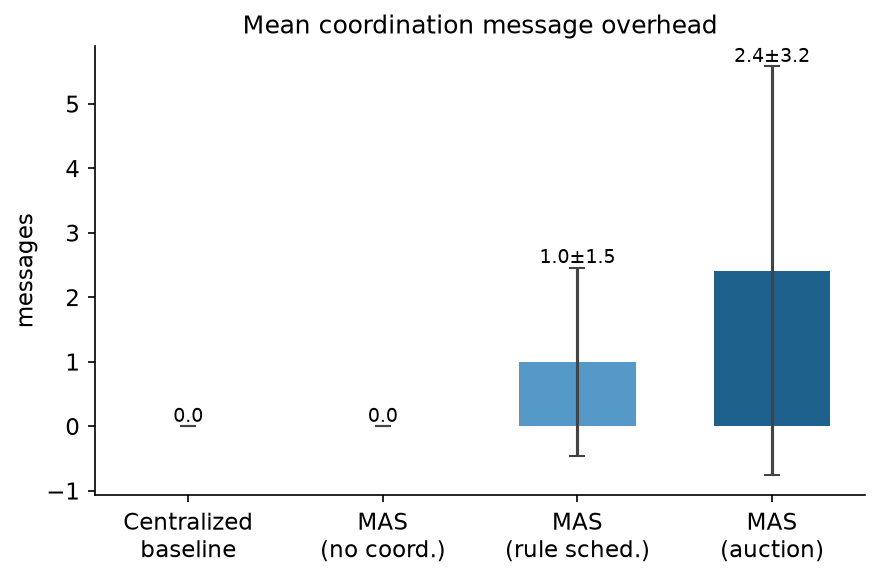
\includegraphics[width=0.7\textwidth]{Assets/fig_coordination_overhead.png}
	\caption{Coordination message overhead per run, counted as in-process bus publications.}
	\label{fig:coordination_overhead}
\end{figure}

RQ2 remains unresolved. The protocol is implemented, terminates, and has a bounded, measured message count. The experiment does not test whether utility-based allocation outperforms arbitrary allocation because the utility function's informative term was inactive.

\section{Discussion}

\subsection{Interpretation}

The first version attributed responsiveness to concurrency and stability to market-based coordination. The corpus-wide data do not support either claim. The latency result is confined to one scenario and is not significant; the stability result fails its homogeneity test.

The evaluation supports three narrower observations:

\begin{enumerate}
	\item \textbf{Architecture choice is not resolved as the main source of detection quality.} The four coordination topologies have statistically indistinguishable F1 over nine scenarios. Variation between scenarios is larger than variation between modes (Figure~\ref{fig:per_scenario_f1}).
	\item \textbf{Representation choices affected the measured score.} The audio-backend result comes from the label space, not the coordination topology: an output type that cannot match a ground-truth family scores zero. The cross-modal confidence result is similarly limited by saturation in the confidence representation.
	\item \textbf{Several mechanisms were inactive during measurement.} The overlap term in the bid, the \gls{mqtt}/Redis substrate, and the \gls{llm} explanation path were not exercised in the reported runs. Comparing code with artifacts exposed those gaps.
\end{enumerate}

The evaluation apparatus is the clearest contribution of this thesis. Fresh-subprocess isolation, repetition indices, the preserved pre-fix baseline CSV, the methodology-change log in Appendix~\ref{app:methodology}, and the inferential analysis exposed results that a single favourable run did not show.

\subsection{Threats to Validity and Limitations}
\label{sec:threats}

\textbf{Pacing confound (internal validity).} \texttt{scenarios/replay.py} sets \texttt{realtime = mode != "centralized"}, so MAS modes pace playback to source frame rate while the centralized baseline runs unpaced and processes sensors sequentially to completion. Because \texttt{FusionAgent.window\_seconds} and \texttt{PolicyAgent.cooldown\_seconds} are wall-clock quantities, the effective temporal width of the fusion window and the alert cooldown differ between modes. The RQ1 latency comparison therefore measures pacing policy together with architecture, and is not attributable to architecture alone. A paced centralized variant is the required control and was not run.

\textbf{Strawman baseline (construct validity).} A production video-management system ingests streams concurrently at real time; it does not process them one after another to completion. The sequential baseline is weaker than the real comparator, which biases RQ1 in the MAS variants' favour by construction.

\textbf{Family-level matching cannot distinguish event types.} The matcher compares incident \emph{families}, and the taxonomy assigns \texttt{intrusion}, \texttt{loitering}, \texttt{abandoned\_object}, and \texttt{audio\_glass\_break} all to \emph{security}. On \texttt{demo\_site\_01}, whose three ground-truth entries are all in that family, an \texttt{intrusion} alert can satisfy the \texttt{loitering} entry. The metric answers ``did some security-relevant alert occur near this time,'' not ``was the right event detected.''

\textbf{Tolerance width.} Matching accepts $[t_{start}-5,\,t_{end}+5]$. For \texttt{demo\_site\_01}'s intrusion interval $[3,35]$ on a 55~s scenario, the acceptance window spans roughly 73\% of the run, which limits how much information precision, recall, and TTA can carry on that scenario.

\textbf{Greedy assignment under-credits successful fusion.} The matcher is a first-fit loop over ground truth in manifest order, not an optimal assignment. On \texttt{combined\_audio\_video\_01}, whose manifest lists \texttt{intrusion} before \texttt{audio\_glass\_break} (both \emph{security}), a single successfully-fused alert satisfies the first entry and leaves the second unmatched, capping measured recall below what the system achieved. A Hungarian assignment would remove the order dependence.

\textbf{FA/h is degenerate at these run lengths.} False alerts per hour is $fp/(\text{wall seconds}/3600)$. With runs as short as 9.1~s and false-positive counts in $\{0,1,2,3\}$, the metric reaches 393.9 alerts/hour from a single false positive. Figure~\ref{fig:fa_per_hour_degeneracy} shows the measured values lying exactly on the $fp\times3600/\text{duration}$ hyperbolae: the statistic reports run duration as much as alert quality, and should not be read as an operational false-alarm rate.

\begin{figure}[H]
	\centering
	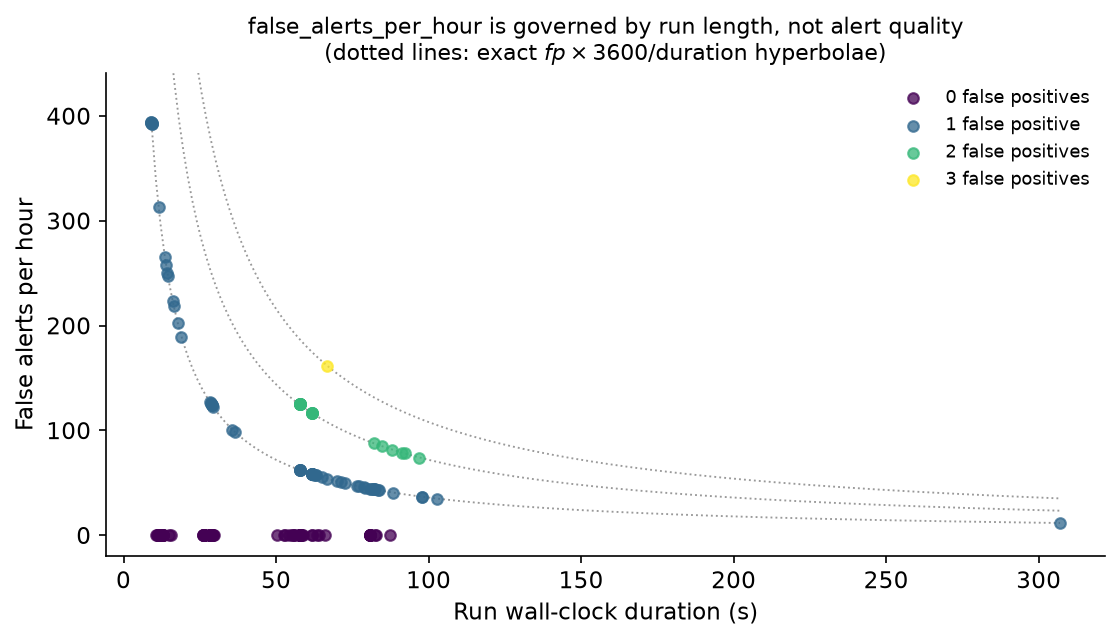
\includegraphics[width=0.82\textwidth]{Assets/fig_fa_per_hour_degeneracy.png}
	\caption{False alerts per hour against run duration. Every point lies on an exact hyperbola determined by its integer false-positive count, showing the metric is governed by the denominator.}
	\label{fig:fa_per_hour_degeneracy}
\end{figure}

\textbf{Known-false ground truth on the demonstrator scenario.} \texttt{scenarios/loitering\_01.json} records an empirical check on the same clip and zone: the longest continuous single-track presence is 5.5~s, below the 8~s loitering threshold, so the loitering event \texttt{demo\_site\_01} declares at $t=16$--$46$~s is not detectable by the implemented rule. That entry remains in the manifest and mechanically caps recall at $2/3$; 48 of 60 \texttt{demo\_site\_01} rows show exactly one false negative. The numbers in this chapter are reported with the annotation in place, and it should be regarded as a known defect of that scenario rather than a system limitation.

\textbf{Verification examines the wrong frame.} \texttt{CameraAgent.\_verify()} re-analyses \texttt{self.\_last\_frame}, the most recent frame read, whereas the hypothesis under verification was formed from events up to 6~s earlier plus the bid window. Under real-time pacing the verified frame typically postdates the incident. The field is also written by the camera thread and read by the coordinator's callback thread without synchronization. Additionally, \texttt{\_verify()} counts only \texttt{person} detections regardless of hypothesis type, so verifying an \texttt{abandoned\_object} or \texttt{audio\_alarm} hypothesis asks a question unrelated to that hypothesis.

\textbf{Semantic anomaly calibration.} The \gls{clip} zero-shot anomaly scorer measures \gls{auc}~$=0.308$ against held-out labelled frames---\emph{worse than a random classifier}---root-caused to a prompt/scene domain mismatch: the normal prompts describe indoor warehouse scenes while much of the corpus is outdoor street footage. Because \gls{clip} usage is held constant across all four variants, this does not bias the relative architectural comparison, but it means the semantic-anomaly channel contributed an anti-correlated signal, and no claim about \gls{clip}'s standalone usefulness in this deployment is warranted.

\textbf{Unjustified parameters.} More than twenty constants govern the decision path---modality weights $0.9/0.7$, bonuses $0.05$, window 6~s, gray zone $[0.35,0.75)$, thresholds $0.45/0.55/0.70$, cooldown 20~s, verification $\pm0.15/-0.20$, tolerance $\pm5$~s, dwell 8~s, static 10~s, \gls{iou} 0.6, and the per-class audio thresholds (Appendix~\ref{app:config}). None was tuned on a held-out split and only the \gls{clip} anomaly threshold was swept. No sensitivity analysis is offered, so the reported operating point should be treated as one arbitrary point in a large unexplored space.

\textbf{No seed control.} No random seed, thread count, or determinism flag is set anywhere. Run-to-run variation was observed and is handled by repetition rather than elimination, which inflates the variance against which all effects are measured and thus further reduces power.

\textbf{Scale.} Nine scenarios, at most three sensors, and runs of 8--73~s. Absolute values are demonstrator-scale; the corpus is too small to resolve the effects the research questions ask about, as Section~\ref{sec:power} quantifies.

\subsection{The Demonstrator Scenario as a Case Study}
\label{sec:demo_case}

\texttt{demo\_site\_01} remains useful as an illustration of the full pipeline exercising every mechanism---multi-sensor concurrency, cross-modal fusion, gray-zone verification, thresholds, cooldowns, anonymization, and explanation---within a single 55~s replay. Table~\ref{tab:ablation} reproduces its per-mode results for that purpose.

\begin{table}[H]
	\centering
	\caption{Single-scenario results on \texttt{demo\_site\_01} ($N=5$; mean$\pm$sd). \textbf{Retained as an illustrative case study only.} These values are not representative of the corpus: see Table~\ref{tab:per_scenario_f1} and Section~\ref{sec:power}.}
	\label{tab:ablation}
	\small
	\begin{tabular}{lcccccc}
		\toprule
		\textbf{Mode} & \textbf{F1}     & \textbf{Precision} & \textbf{Recall} & \textbf{TTA (s)} & \textbf{FA/h} & \textbf{Msgs} \\
		\midrule
		Centralized   & 0.773$\pm$0.059 & 0.933$\pm$0.149    & 0.667$\pm$0.000 & 15.07$\pm$3.11   & 7.4$\pm$16.5  & 0             \\
		MAS-nocoord   & 0.781$\pm$0.204 & 0.767$\pm$0.224    & 0.800$\pm$0.182 & 5.60$\pm$3.14    & 29.8$\pm$36.5 & 0             \\
		MAS-rules     & 0.629$\pm$0.053 & 0.600$\pm$0.091    & 0.667$\pm$0.000 & 3.64$\pm$0.27    & 61.4$\pm$21.4 & 2$\pm$0.0     \\
		MAS-auction   & 0.667$\pm$0.000 & 0.667$\pm$0.000    & 0.667$\pm$0.000 & 2.96$\pm$0.14    & 52.6$\pm$5.9  & 5$\pm$0.0     \\
		\bottomrule
	\end{tabular}
\end{table}

Read as a case study, this scenario is instructive precisely because it is misleading in isolation: it is the one scenario where the MAS latency advantage is large, the one where a known-false ground-truth entry caps recall, and the one whose three ground-truth events all collapse into a single incident family. It is a good demonstration and a poor experiment, and the distinction is the methodological lesson of this chapter.

Figures~\ref{fig:detection_quality} and \ref{fig:system_metrics} present the corpus-pooled detection-quality and responsiveness views retained from the first version, now understood in light of the inferential analysis above.

\begin{figure}[H]
	\centering
	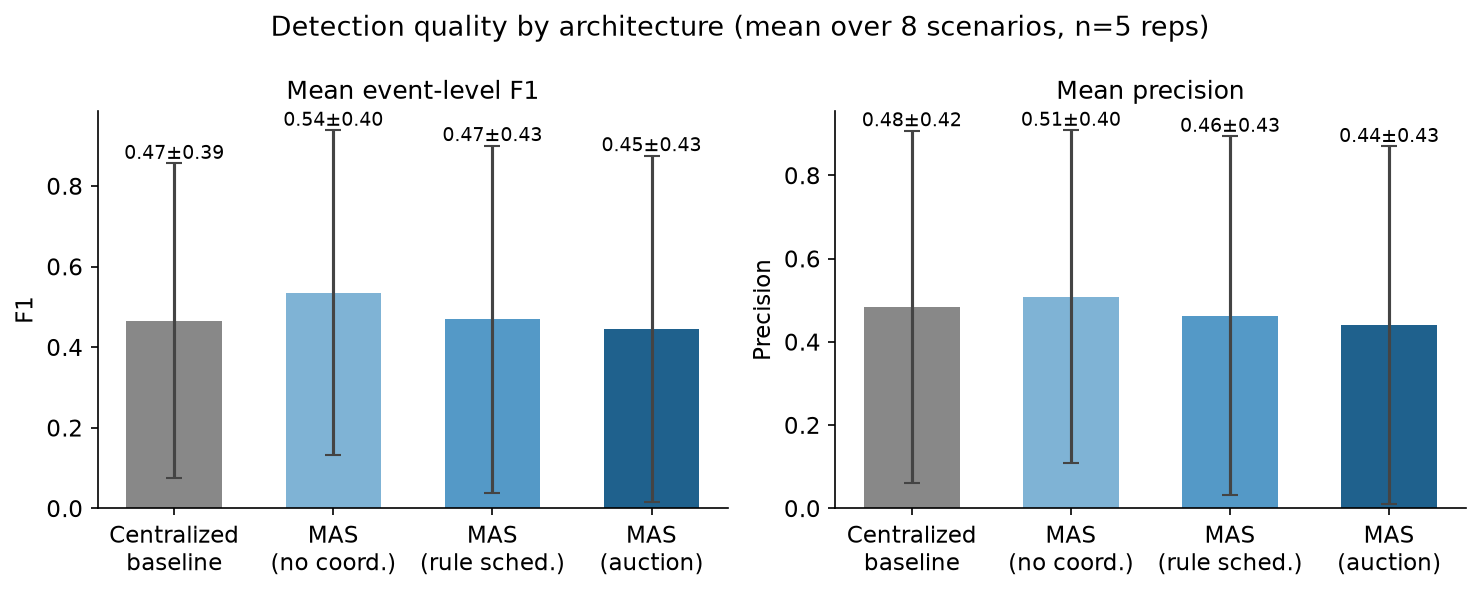
\includegraphics[width=0.85\textwidth]{Assets/fig_detection_quality.png}
	\caption{Detection quality pooled across scenarios and repetitions (error bars are pooled sample standard deviations, not confidence intervals; cf.\ Figure~\ref{fig:mode_ci}).}
	\label{fig:detection_quality}
\end{figure}

\begin{figure}[H]
	\centering
	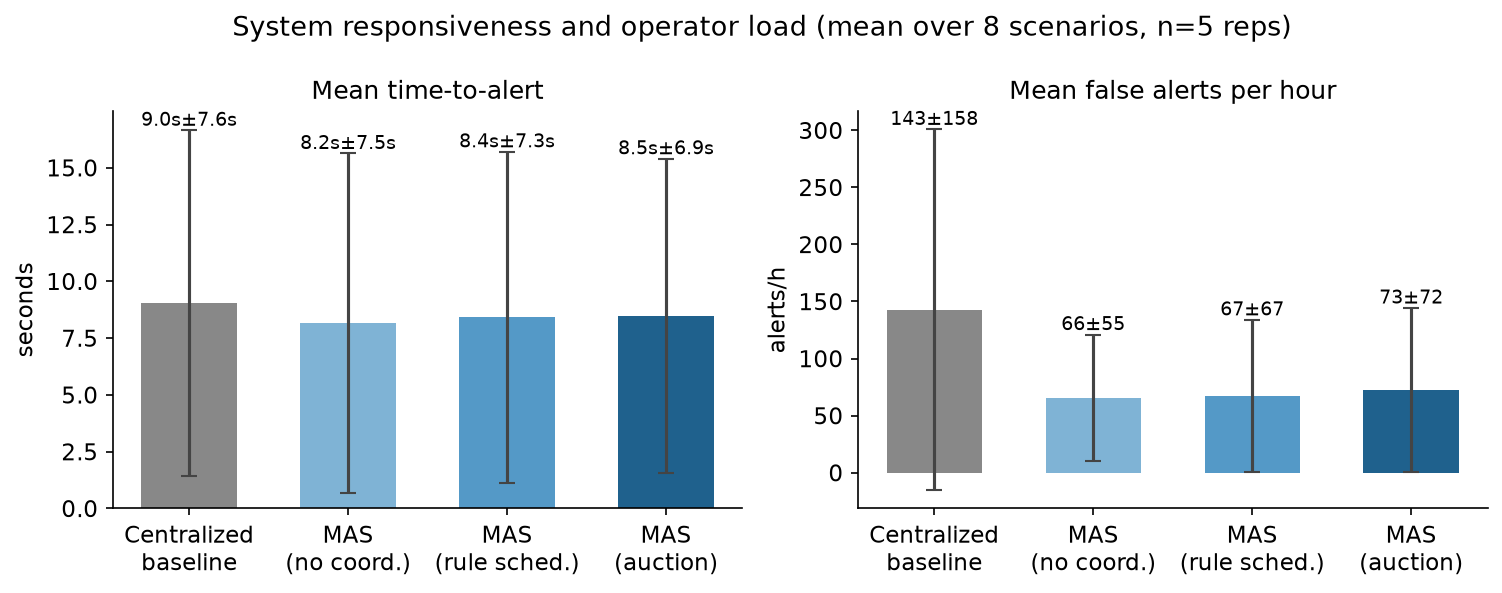
\includegraphics[width=0.95\textwidth]{Assets/fig_system_metrics.png}
	\caption{Pooled time-to-alert and false alerts per hour. The FA/h panel should be read with Figure~\ref{fig:fa_per_hour_degeneracy} in mind.}
	\label{fig:system_metrics}
\end{figure}

\begin{figure}[H]
	\centering
	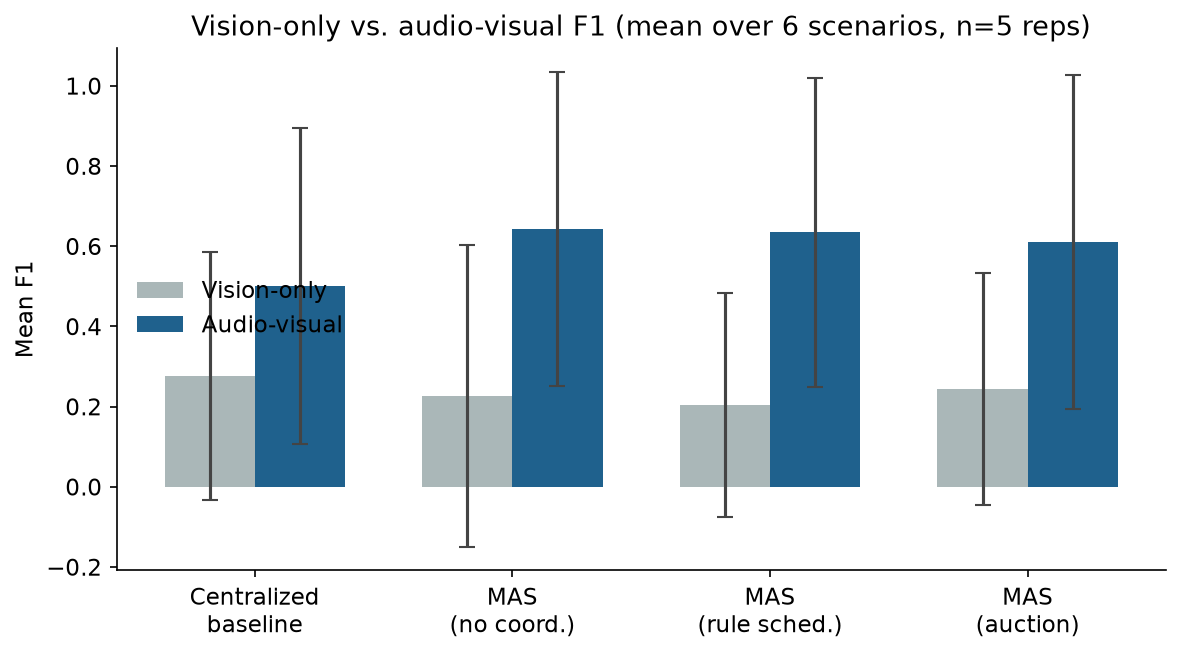
\includegraphics[width=0.85\textwidth]{Assets/fig_modality_ablation.png}
	\caption{Vision-only versus audio-visual F1 across the audio-capable scenarios.}
	\label{fig:modality_ablation}
\end{figure}

\section{Conclusion}

Across nine scenarios and 373 runs, the hierarchical \gls{mas} is not demonstrably faster to alert than the centralized pipeline once more than one scenario is considered. Pacing confounds RQ1. Auction coordination is not shown to improve precision or false-alert rate, and its central mechanism was inactive during measurement, so RQ2 remains unresolved. Cross-modal fusion works, but noisy-OR saturation makes its confidence contribution unmeasurable and cross-modal alerts are rare. The explanation guardrail is structurally supported and fired on the single real-model run, but the campaign did not exercise it. The privacy and audit pipeline held across all 373 runs, although anonymization efficacy was not measured.

Three research questions remain negative or unresolved. The replay artifacts, repeated runs, and inferential analysis made those limits visible. The final chapter revises the contribution claims and identifies the work needed to answer the open questions.
